\part{Working with R}
% ------------------------------------------------------------
%---
% %%%%%%%%%%%%%%%%%%%%%%%
% \section{Saving Plots as a PDF} 
% %%%%%%%%%%%%%%%%%%%%%%%
% \begin{frame}[fragile]
% \frametitle{Saving Plots as a PDF}
%   \framesubtitle{For Static Plots}

%   \itshape Note: \normalfont The files will be saved in the folder specified with \ttfamily setwd(). \normalfont
%   To save a static plot in \ttfamily R \normalfont as a PDF, use function \ttfamily pdf(): \normalfont

%   \begin{lstlisting}
% # To save the image to the desktop:
% setwd("~/Desktop")
% pdf("filename.pdf")
% wireframe(volcano, col.regions = terrain.colors(100), asp = 1, color.key=TRUE, drape=TRUE, scales = list(arrows = FALSE))
% dev.off()
%   \end{lstlisting}

% \end{frame}

% \begin{frame}[fragile]
%   \frametitle{Saving Plots as a PDF}
%   \framesubtitle{For Dynamic Plots}

%   \itshape Note: \normalfont The files will be saved in the folder specified with \ttfamily setwd(). \normalfont
%   To save a dynamic plot in \ttfamily R \normalfont as a PDF, use function \ttfamily rgl.snapshot(): \normalfont

%   \begin{lstlisting}
% # To save the image to the desktop:
% setwd("~/Desktop")
% # Step 1: Produce the 3D image:
% plot3d(x=quakes$long, y=quakes$lat, z=quakes$depth, xlab="Longitude", ylab="Latitude", zlab="Depth")
% # Step 2: Can rotate before taking a snapshot:
% rgl.snapshot("quakes.png")
%   \end{lstlisting}

% \end{frame}

%%%%%%%%%%%%%%%%% 
\section{Common Bugs and Fixes}
%%%%%%%%%%%%%%%%%%%%%%%%%%%%%%%%%%%%%

\subsection{Syntax Error}
\begin{frame}[fragile]
  \frametitle{\ttfamily Error: syntax error \normalfont}
Possible causes:
  \begin{itemize}
    \item Misspelling the object's name
    \item Including a "$+$" when copying code from console/website, etc.
    \item Having an extra parenthesis at the end of a function
    \item Having an extra bracket when subsetting
  \end{itemize}
\end{frame}

\subsection{Trailing $+$}
\begin{frame}[fragile]
  \frametitle{Trailing $+$}
Possible causes:
  \begin{itemize}
    \item Not closing a function call with a parenthesis
    \item Not closing brackets when subsetting
    \item Not closing a function you wrote with a squiggly brace
  \end{itemize}
\end{frame}

\subsection{Error When Performing Operations}
\begin{frame}[fragile]
  \frametitle{\ttfamily Error in ... : requires numeric matrix/vector arguments \normalfont}
Possible causes:
  \begin{enumerate}
    \item Objects are data frames, not matrices
    \item Elements of the vectors are characters \\
  \end{enumerate}
  
Possible solutions:
  \begin{enumerate}
    \item Coerce (a copy of) the data set to be a matrix, with the \ttfamily as.matrix() \normalfont command
    \item Coerce (a copy of) the vector to have numeric entries, with the \ttfamily as.numeric() \normalfont command
  \end{enumerate} 
\end{frame}

\subsection{Error in Calling an Object}
\begin{frame}[fragile]
  \frametitle{\ttfamily Error: ... object not found \normalfont}
Possible causes:
  \begin{enumerate}
    \item Misspelling the object's name
    \item Package containing the object has not been loaded
  \end{enumerate}
  
\end{frame}

\subsection{Silent Errors}
\begin{frame}[fragile]
  \frametitle{Silent Errors}
Most common silent errors:
  \begin{enumerate}
    \item (Inadvertently) Creating a data set with no rows or columns. 
    \item (Inadvertently) Recycling (and padding) of entries in a variable with a smaller number of observations than the one it is compared to.  
  \end{enumerate}
Possible solutions:
  \begin{enumerate}
    \item Always check the dimensionality of the data set after subsetting.
    \item Always check the lengths of variables ahead of comparison, especially if subsetting just took place.
  \end{enumerate}   
\noindent For more caveats and solutions, read the "R Inferno": \url{http://www.burns-stat.com/pages/Tutor/R_inferno.pdf}
  
\end{frame}

%%%%%%%%%%%%%%%%%%%%%%%%%%%%%%%%%%%%%
% Section: Wher to go from here?
\section[Next Steps]{Where to go from here?}
%%%%%%%%%%%%%%%%%%%%%%%%%%%%%%%%%%%%%
\begin{frame}
  \frametitle{Where to go fom here?}
  \framesubtitle{Part 1: Explore other visualizations}

  Other exploratory visualizations in R that we didn't get to cover:
  \begin{itemize}
    \item Sankey graphs
    \item (Interactive) dashboards via R package 'shiny'   
    \item Creating animations with R
    \item $\cdots$
  \end{itemize}
\end{frame}

%--- 
\begin{frame}
  \frametitle{Where to go fom here?}
  \framesubtitle{Part 2: Familiarize yourself with R (as it relates to EDA)}

  Other data-related topics that we didn't get to cover:
  \begin{itemize}
    \item Variety of ways to aggregate data
    \item Getting data via an API (e.g. meetup, yelp, etc.)
    \item Developing reproducible reports (via 'knitr' package)    
    \item $\cdots$
  \end{itemize}
\end{frame}

%--- 
\begin{frame}
  \frametitle{Where to go fom here?}
  \framesubtitle{Part 3: Familiarize yourself with HTML/JS/d3/$\cdots$}

  Other visualization topics that we didn't get to cover:
  \begin{itemize}
    \item Ability to customize design of interactive graphics (e.g. \url{http://datascience.la/interactive-visualizations-from-r-using-rcharts/} and \url{http://www.slideshare.net/f0008/javascriptbased-visualization-in-r})
    \item Ability to customize design of interactive dashboards (e.g. \url{http://shiny.rstudio.com/articles/})
    \item Ability to customize design of reproducible reports   (e.g. \url{http://shiny.rstudio.com/gallery/download-knitr-reports.html}) 
    \item $\cdots$
  \end{itemize}
\end{frame}

%--- 
\begin{frame}
  \frametitle{Where to go fom here?}
  \framesubtitle{Part 4: Familiarize yourself with data analysis models}

  We did not cover model building as a way to explain relationships in the data, such as:
  \begin{itemize}
    \item Different types of regression models for modeling numerical data
    \item Different types of decision trees for modeling numerical data
    \item Different types of models for analyzing text/image/video/audio data   
    \item $\cdots$
  \end{itemize}
  Please see the 'Online Resources for R' section (below) for more information.
\end{frame}

%%%%%%%%%%%%%%%%%%%%%%%%%%%%%%%%%%%%%
% Section: R Help
\section[Help]{Getting R Help}
%%%%%%%%%%%%%%%%%%%%%%%%%%%%%%%%%%%%%

\begin{frame}[fragile]
\frametitle{R Help: Approach 1}

\vspace{-5pt}
For help with any function in R, add a question mark before the function name to see the documentation (which includes explanation of the function's arguments/inputs, function outputs and example use cases.

  \begin{lstlisting}
?plot
  \end{lstlisting}

  \begin{center}
    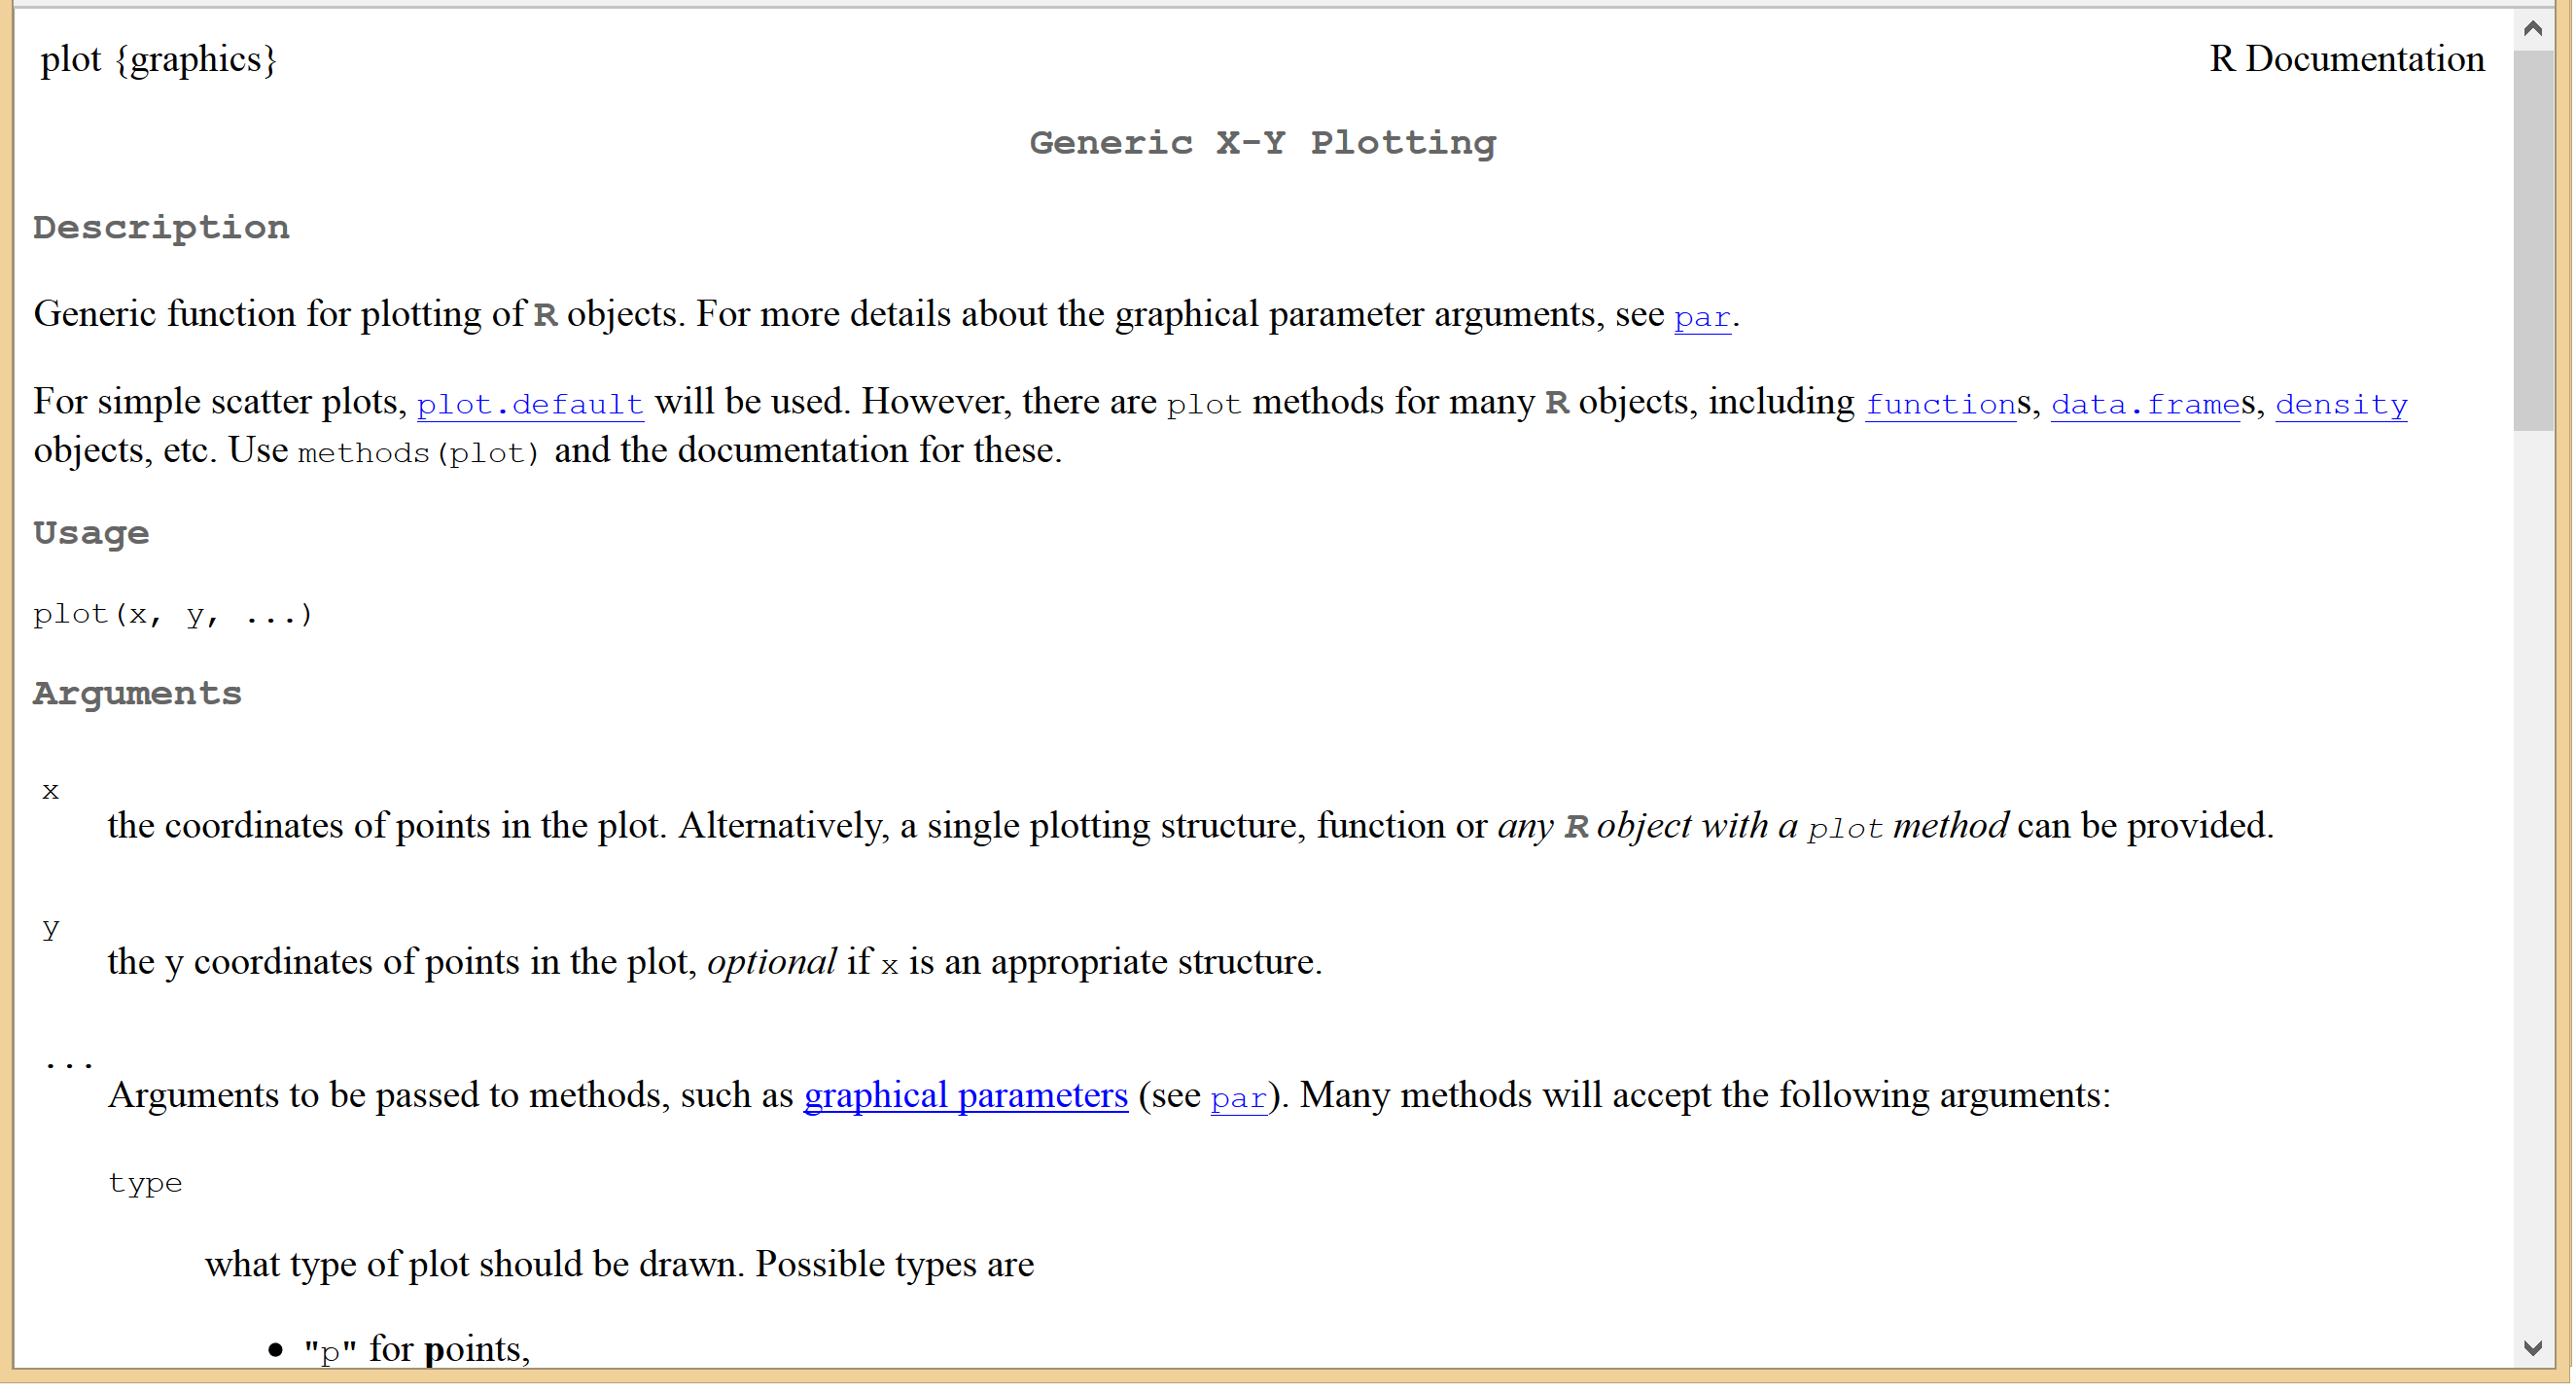
\includegraphics[width=0.6\textwidth]{images/Rhelp}
  \end{center}

\end{frame}
%%%---

\begin{frame}[fragile]
\frametitle{R Help: Approaches 2 and 3}

\vspace{-5pt}
  \begin{itemize}
    \item For help with any function in R, search answers on StackOverflow (SO).
    \item For help with any function in R, when all else fails, ask a question on StackOverflow.  Don't forget to follow the SO tips: \url{http://stackoverflow.com/help/how-to-ask}
  \end{itemize}

  \begin{center}
  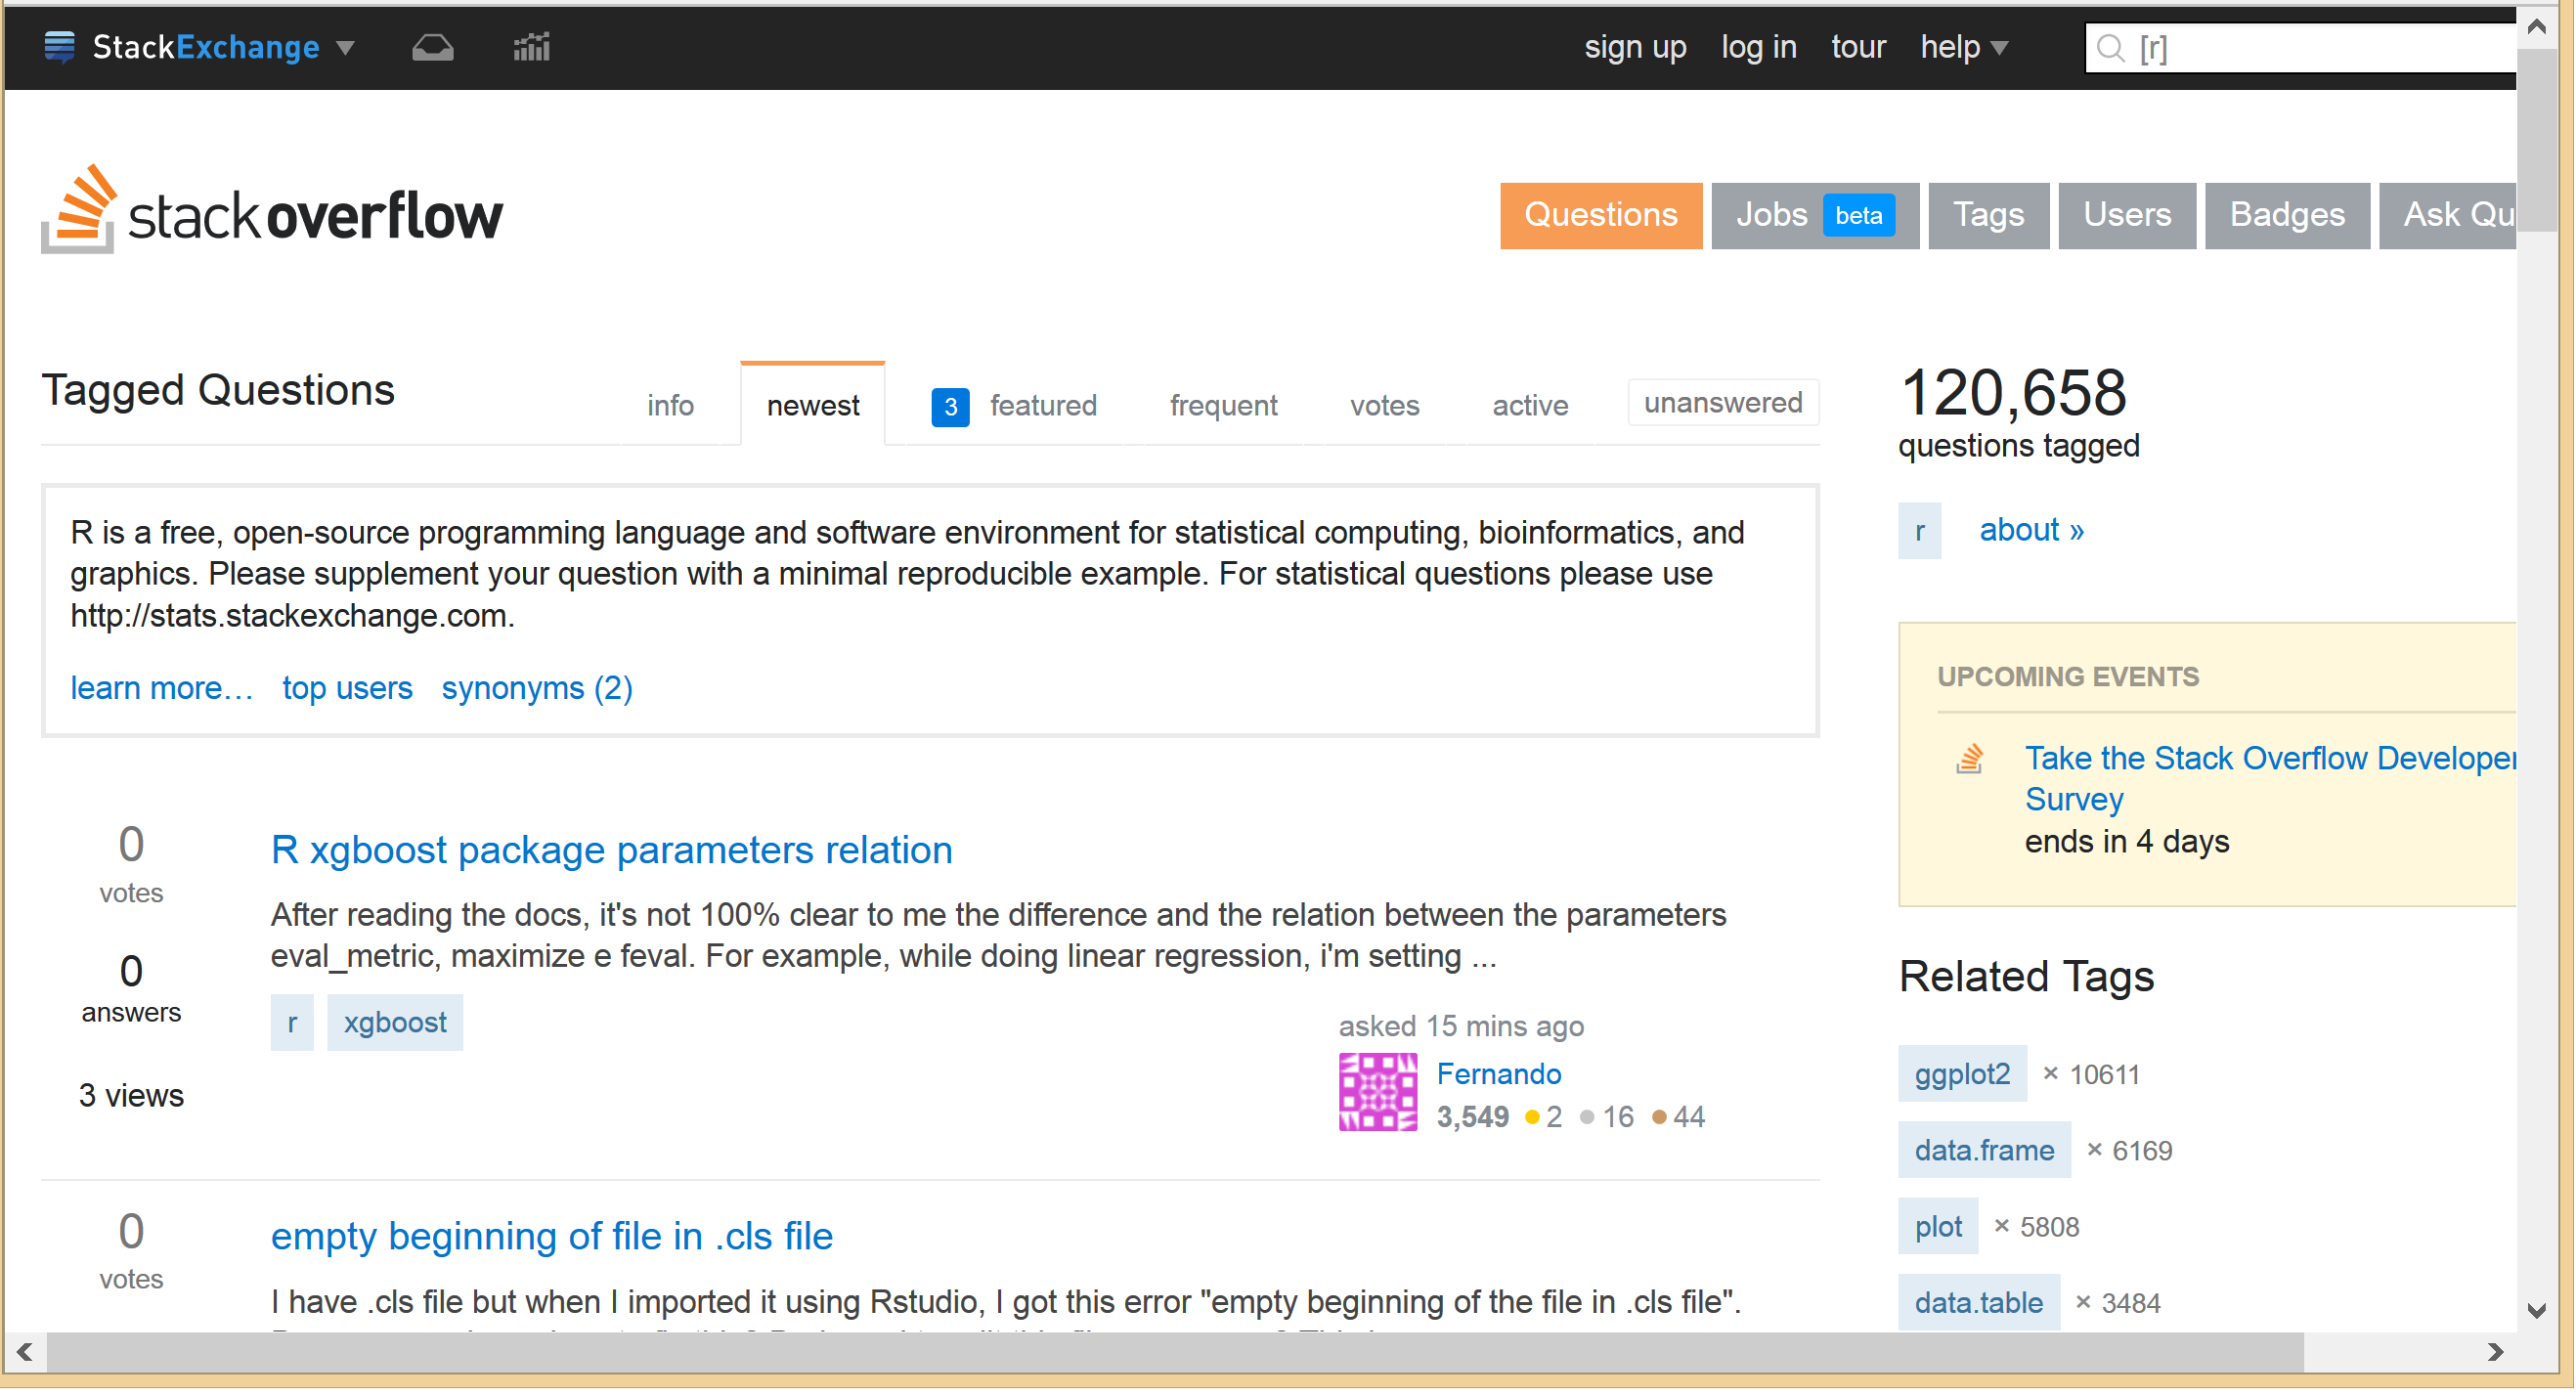
\includegraphics[width=0.65\textwidth]{images/SO}
  \end{center}

\end{frame}



%%%%%%%%%%%%%%%%%%%%%%%%%%%%%%%%%%%%%
%--- Online Resources
%%%%%%%%%%%%%%%%%%%%%%%%%%%%%%%%%%%%%
\section[Online Resources]{Online Resources for R}
\begin{frame}[fragile, allowframebreaks]
  \frametitle{Online Resources for R}
%\begin{description}[<+->] 
%\item[Download R:] http://cran.stat.ucla.edu/
%\item[Search Engine for R:] http://rseek.org
%\item[R Reference Card:] http://cran.r-project.org/doc/contrib/Short-refcard.pdf
%\item[UCLA Statistics Information Portal:] http://info.stat.ucla.edu/grad/
%\item[UCLA Statistical Consulting Center:] http://scc.stat.ucla.edu
%\end{description}

\begin{description}
	\item[Download R:] {\small \textit{\urlwofont{http://cran.stat.ucla.edu/}}}
  \item[Download RStudio:] {\small \textit{\urlwofont{https://www.rstudio.com/}}}  
	% \item[Search Engine for R:] {\small \textit{\urlwofont{http://rseek.org}}}
	\item[R Reference Card:] $\:$ \\
		{\small \textit{\urlwofont{http://cran.r-project.org/doc/contrib/Short-refcard.pdf}}}
	\item[R Graphics Gallery:] $\:$ \\
		 {\small \textit{\urlwofont{http://research.stowers-institute.org/efg/R/}}}
	\item[R Graph Gallery:]  {\small \textit{\urlwofont{http://addictedtor.free.fr/graphiques/}}}
	% \item[UCLA Statistics Information Portal:] \small{ \textit{\urlwofont{http://info.stat.ucla.edu/grad/}}}
	% \item[UCLA Statistical Consulting Center:] \small{ \textit{\urlwofont{http://scc.stat.ucla.edu}}}
  \item[] % Book on R graphics: http://book.flowingdata.com/
  \item[Stackoverflow:] {\small \textit{\urlwofont{http://stackoverflow.com/tags/r/info}}}
  \item[Blogs:] {\small \textit{\urlwofont{http://www.r-bloggers.com/}}}
  \item[JSS:] {\small \textit{\urlwofont{https://www.jstatsoft.org/index}}}
  \item[More R tutorials:] 
    \begin{itemize}
      \item[]
      \item[Courses:] Code School, Coursera, DataCamp, DataRobot, edX, RStudio, swirl
      \item[IK:] {\small \textit{\urlwofont{http://www.KukuyevaConsulting.com/tutorials}}}
      \item[UCLA IDRE:] {\small \textit{\urlwofont{http://www.ats.ucla.edu/stat/r/}}}
      \item[UCLA SCC:] {\small \textit{\urlwofont{http://scc.stat.ucla.edu/mini-courses/}}}
    \end{itemize}  
 \end{description}
\end{frame}


% http://adv-r.had.co.nz/ 
% http://www.statmethods.net/interface/packages.html package install
% List of packages https://cran.r-project.org/web/packages/
% Gallery: http://rgraphgallery.blogspot.com/search/label/barchart
% Steam charts: http://www.r-bloggers.com/data-mountains-and-streams-stacked-area-plots-in-r/

%%%%%%%%%%%%%%%%%%%%%%%%%%%%%%%%%%%%%
\section{References}
%%%%%%%%%%%%%%%%%%%%%%%%%%%%%%%%%%%%%

\begin{frame}[allowframebreaks]
  \begin{itemize}
    \item[1.] \url{http://adv-r.had.co.nz/}
    \item[2.] \url{http://www.sixhat.net/how-to-plot-multpile-data-series-with-ggplot.html}
    \item[3.] \url{http://stackoverflow.com/questions/17584248/exact-axis-ticks-and-labels-in-r-lattice-xyplot}
    \item[4.] \url{https://rstudio-pubs-static.s3.amazonaws.com/3364_d1a578f521174152b46b19d0c83cbe7e.html}
    \item[5.] \url{www.jstatsoft.org/v25/c01/paper}
    \item[6.] \url{http://www.kdnuggets.com/2015/05/r-vs-python-data-science.html}
    \item[7.] \url{http://flowingdata.com/2014/02/05/where-people-run/}
    % \item[8.] \url{http://xkcd.com/688/}
    \item[8.] \url{https://www.facebook.com/notes/facebook-engineering/visualizing-friendships/469716398919}
    \item[9.] Iliinsky, N. and Steele, J. (2011) \itshape{Designing Data Vizualizations} \normalfont Sebastopol, CA: O'Reilly.
    \item[10.] \url{http://www.pixel-push.com/2013/09/24/ultimate-infographic-resource-kits-for-designers/}
    \item[11.] Heiberger, R. M. (2016, February). Design of Not-Simple Graphs. Talk presented at the 
     meeting of the American Statistical Association Conference on Statistical Practice, San Diego, CA.
     \item[12.] \url{https://github.com/hadley/ggplot2/wiki/plotting-polygon-shapefiles}
     \item[13.] \url{http://www.r-bloggers.com/making-static-interactive-maps-with-ggvis-using-ggvis-maps-wshiny/}
  \end{itemize}
\end{frame}

%_________________________________ Part
%%%%%%%%%%%%%%%%%% Section: Exercise

%\frame{
%  \frametitle{Upcoming Mini-Course}
%	\framesubtitle{This Wednesday}
%$4:30$PM: Advanced Graphics with \ttfamily R \normalfont
%}

\frame{
  \frametitle{}
\begin{center}
Thank you.\\

Any questions?
\end{center}
}